\section{Pipeline for Static Input}
\label{sect:pipeline-for-static-input}

For static input graphs our pipeline looks as follows: In a first step, we determine clusters of vertices in the input graph and their relationships (similarities). We then pick the most important relationships we want our visualization to show and determine some combinatorial arrangement of the clusters. We transform this embedding into an equivalent contact representation whose faces are represent the clusters and whose adjacencies represent the clusters' relationships. Eventually, we optimize the contact representation such that the areas are (close to) proportional to the cluster weights, \ie{} the number of vertices in the clusters. The contact representation essentially is the area-proportional map we want to create.

The following figure depicts a rough sketch of the phases and intermediate products of the pipeline for static inputs:

\begin{figure}[H]
	\centering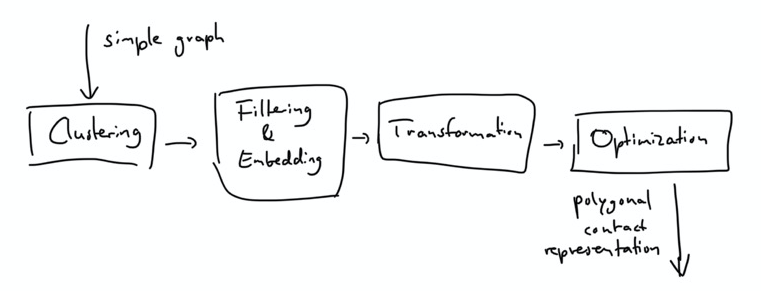
\includegraphics[height=140px]{Resources/Pipeline-Static.png}
	\caption{Overall structure of the static pipeline.}
	\label{fig:pipeline-static}
\end{figure}

We will now discuss the individual phases of the pipeline in greater detail.



\subsection{Clustering Phase}

In the first step of the pipeline, we cluster the input graph. We take the static, simple input graph and compute clusters of vertices and their similarities. This yields a complete vertex- and edge-weighted graph that we call the \emph{clustered graph}.

\begin{figure}[H]
	\centering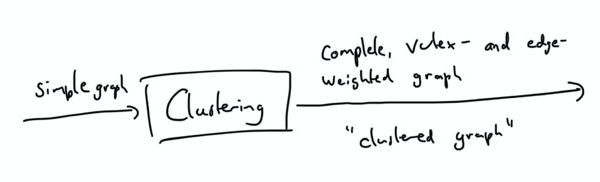
\includegraphics[height=100px]{Resources/Pipeline-Clustering.png}
	\caption{Input and output of the \quoted{Clustering} phase.}
	\label{fig:pipeline-static}
\end{figure}

Vertices in the clustered graph correspond to clusters in the primal graph and are weighted by the size of the corresponding clusters, \ie{} the number of vertices in the clusters. Edges in the clustered graph represent the similarity of two clusters, \ie{} the number of edges going from one cluster to the other, and are weighted accordingly. Without loss of generality we assume the cluster graph to be complete, meaning that an edge exists between every pair of vertices \emdash{} missing edges can simply be added with a weight of zero.

The clustered graph is the foundation of the map we are going to create: its vertices and their weights are the regions and their desired areas of the map. A subset of its edges will be represented in the map by the border between two countries.

% and complete graphs on 4 or more vertices are not planar.
%, though we won't be able to visualize every edge of the clustered graph, as we'll see in the next phase.



\subsection{Filtering and Embedding Phase}

In the second step we determine the overall structure that the map is going to have. To understand the requirements of this step, we need the concept of (k-)map graphs and planar graphs.

A \emph{map graph} is defined as the intersection graph of a finite number of mutually internally disjoint regions of the plane, \ie{} its vertices are the regions and two vertices are connected by an edge if their regions touch \cite{chen2002map}. For map graphs, the number of regions that can meet in a point is unlimited, allowing for large cliques in map graphs. Although not unlimited, there are cases where more than 3 regions meet in a point in real-world maps, such as the Four Corners (Colorado, Utah, Arizona, New Mexico) in the United States.

\emph{Planar graphs} are graphs that can be drawn on the plane without its edges crossing, or, more specifically, with its edges intersecting only at their endpoints \cite{wagner2016algorithmen}. There is an equivalent definition that is remarkably similar to the one of map graphs above, namely a planar graph is a graph whose vertices are mutually internally disjoint regions of the plane, in which two vertices are adjacent iff the respective regions share an edge, \ie{} more than just a single point \cite{chen2002map}. Obviously planar graphs are a subclass of map graphs because they have stricter requirements.

In this thesis, we want to create maps that induce planar graphs. Note that in the definition of  planar graphs we start with regions in the plane and turn them into a graph. We'll want to go in the opposite direction here: we already have a planar graph and want to turn it into mutually internally disjoint regions whose adjacencies are equivalent to those of the vertices in the graph.

First of all, we'll need to filter the clustered graph from the previous step: complete graphs on 4 or more vertices aren't planar \cite{wagner2016algorithmen}, but we can decide on a planar subgraph of the order, \ie{} the same number of vertices, by filtering out a couple of edges. However, the graph should remain 2-connected and internally triangulated for reasons we'll outline below. Note that triangulated graphs are planar by definition.

If the graph wasn't internally triangulated, it would have holes, \ie{} internal faces on 4 or more vertices. In a corresponding map, this hole would result in lakes or rivers, which are artifacts we do not want.

\begin{figure}[H]
	\centering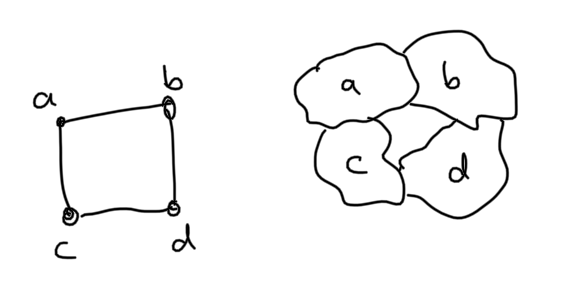
\includegraphics[height=120px]{Resources/Filtering-Hole.png}
	\caption{A 4-hole (left) and a corresponding contact representation (right).}
	\label{fig:filtering-holes}
\end{figure}

We also restrict ourselves to 2-connected graphs such that, in combination with the internal triangulated requirement, the outer face doesn't contain a vertex multiple times. This is due to a detail in our concrete implementation that we'll discuss later and is a restriction that could be lifted in future research.

\begin{figure}[H]
	\centering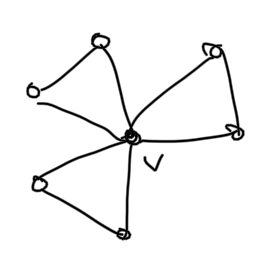
\includegraphics[height=120px]{Resources/Filtering-Connectedness.png}
	\caption{A forbidden graph with a cut vertex $v$.}
	\label{fig:filtering-connectedness}
\end{figure}

Most importantly, we also decide on one of potentially many different combinatorial embeddings of the filtered graph. A \emph{combinatorial embedding} defines the cyclic orders of incident edges around the graph's vertices. \Cref{fig:filtering-embedding} shows how different combinatorial embeddings of the same graph can have vastly different appearances. Choosing a  combinatorial embedding essentially locks in the overall structure or the resulting map.
%In dynamic context: crucial to preserve mental map!

\begin{figure}[H]
	\centering
	\subfigure[clockwise]{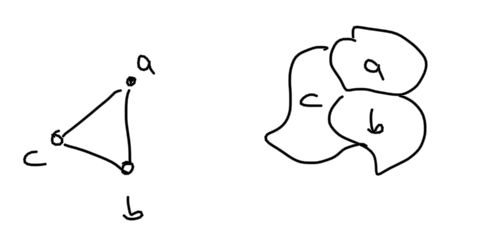
\includegraphics[width=60mm]{Resources/Filtering-Embedding-Clockwise.png}}
	\subfigure[counterclockwise]{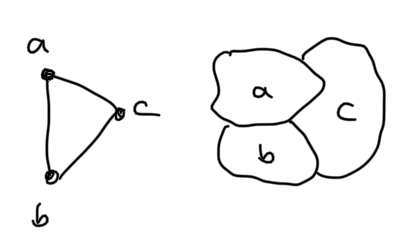
\includegraphics[width=60mm]{Resources/Filtering-Embedding-Counterclockwise.png}}
	\caption{A triangle embedded both clockwise and counterclockwise and the different resulting maps.}
	\label{fig:filtering-embedding}
\end{figure}

In summary, we take the clustered graph and filter out edges to create a vertex- and edge-weighted, 2-connected, and internally triangulated subgraph with the same number of vertices, and decide on a combinatorial embedding which we'll refer to as the \emph{filtered graph embedding}. Typically you'd want to preserve the edges with the highest weights, but other implementations are possible as well.

\begin{figure}[H]
	\centering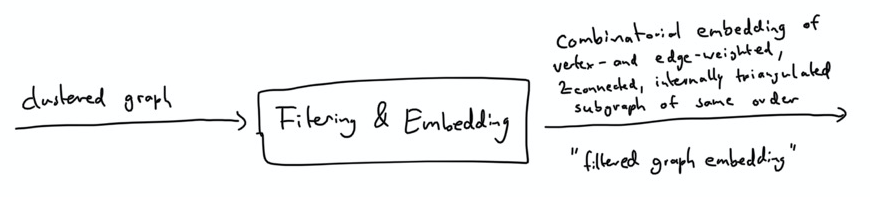
\includegraphics[width=0.9\textwidth]{Resources/Pipeline-Filtering-and-Embedding.png}
	\caption{Input and output of the \quoted{Filtering \& Embedding} phase.}
	\label{fig:pipeline-static}
\end{figure}


\subsection{Transformation Phase}

In the third phase, we take the filtered graph embedding and turn it into a valid map.

Formally speaking, the map we want to create is an area-proportional contact representation of the filtered graph embedding: The regions on the map correspond to the vertices of the filtered graph embedding and the clusters in the primal graph. Neighboring regions represent edges of the filtered graph embedding and the similarity of two clusters in the primal graph.

In this thesis we restrict ourselves to simple, polygonal contact representations, \ie{} contact representations in which the regions are polygons that don't intersect themselves. These contact representations can themselves be viewed as topological embeddings of a graph: A graph whose vertices are the endpoints of the polygonal areas and whose edges are the edges of the polygonal areas. We shall refer to this graph embedding as the \emph{boundary graph embedding}. The faces of this graph correspond to vertices in the filtered graph embedding and therefore inherit their weights.

The \emph{dual} of a plane graph $G$ is a pseudograph $G^*$ that has a vertex for each face in $G$, including the outer face, and edges connecting the vertices corresponding to the incident faces of each edge in the primal graph $G$. Forming the dual of a plane graph essentially turns vertices into faces and vice versa and \quoted{flips} the edges of the primal graph. When forming the dual of the dual of a plane graph, we get back the primal graph, \ie{} $(G^*)^* = G$.
%$G^*$ is a pseudograph because it can have loops and parallel edges.
%The dual $G^*$ of a plane graph $G$ is itself plane and an embedding can trivially be derived from an embedding of the primal graph $G$.

The \emph{weak dual} $G^-$ of a plane graph is its dual without the vertex corresponding to the primal outer face \cite{fleischner1974}. We define the \emph{augmented dual} $G^+$ of a plane graph $G$ as the pseudograph obtained by first adding a new vertex in the outer face of $G$ and connecting it to all vertices on the outer face and then forming the dual. By definition, the weak dual of the augmented dual of a plane graph is the primal graph again, \ie{} $(G^+)^- = G$ \cite{fleischner1974}.
\todo{Is there a known name for the inverse of \quoted{weak dual}? I couldn't find anything.}

Using the terminology from above, the filtered graph embedding is the weak dual of the boundary graph embedding with its degree-2-vertices smoothed out. In this phase of the pipeline, we aim to go in the opposite direction though: we are given a filtered graph embedding and want to create a corresponding boundary graph embedding with straight-line edges. We start by forming its augmented dual, as illustrated in the following figure:

\begin{figure}[H]
	\centering
	\subfigure[]{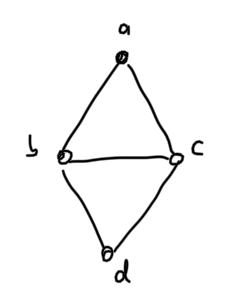
\includegraphics[height=40mm]{Resources/Transformation-1.png}}
	\subfigure[]{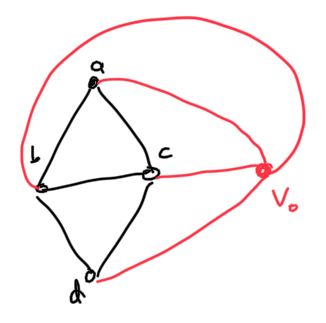
\includegraphics[height=40mm]{Resources/Transformation-2.png}}
	\subfigure[]{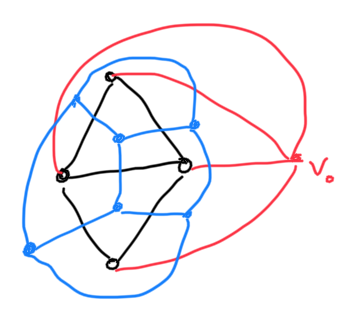
\includegraphics[height=40mm]{Resources/Transformation-3.png}}
	\subfigure[]{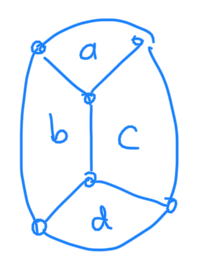
\includegraphics[height=40mm]{Resources/Transformation-5.png}}
	\caption{Step-by-step representation of the transformation from filtered graph embedding (a) to boundary graph embedding (d). We add the helper vertex in red (b) and form the dual in blue (c).}
	\label{fig:transformation}
\end{figure}

Since the boundary graph is supposed to have straight-line edges, we may need to tweak the embedding to straighten out the edges. The boundary graph is simple by definition, \ie{} it has no loops or parallel edges. Thus according to Fáry's theorem \cite{fary1948straight}, there exists a combinatorially isomorphic, straight-line re-embedding of the graph.

Thomassen proved that there exist straight-line drawings of all plane cubic graphs with arbitrary prescribed face areas \cite{thomassen1992plane}. Adding a new vertex in the outer face of an internally triangulated graph and connecting it to all vertices on the outer face creates a fully triangulated graph, and its dual is a cubic (3-regular) graph. Therefore \cite{thomassen1992plane} applies to our boundary graph, meaning that even without any subdivisions there exists an embedding that realizes the face weights, \ie{} a map with perfect statistical accuracy.
% We only need Kleist when lifting restrictions and our graph isn't necessarily cubic.

Such embeddings are non-trivial to find though and may create undesired regions for other quality metrics that we want to optimize for. Concrete implementations of this phase are in no way required to use triangles for all map regions and are free to subdivide edges at will. In fact, we provide a very simple implementation that subdivides all dual edges once and leaves us with enough degrees of freedom to optimize for other quality metrics in \cref{chap:implementation}.

\begin{figure}[H]
	\centering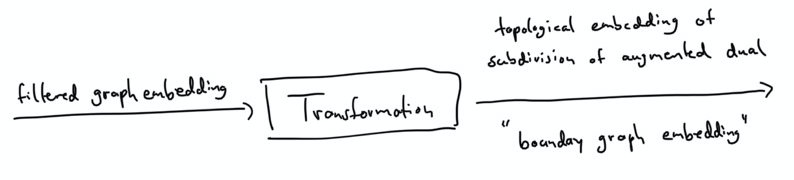
\includegraphics[width=0.9\textwidth]{Resources/Pipeline-Transformation.png}
	\caption{Input and output of the \quoted{Transformation} phase.}
	\label{fig:pipeline-static}
\end{figure}



\subsection{Optimization Phase}

In the fourth and last phase of the pipeline, we improve on the initial drawing of the boundary graph while preserving its combinatorial embedding of the map. We move the vertices around to optimize statistical accuracy and other quality metrics that we are interested in. We can also subdivide edges to create more degrees of freedom or get rid of subdivision vertices (vertices with degree 2) when we don't need those degrees of freedoms any more.

\begin{figure}[H]
	\centering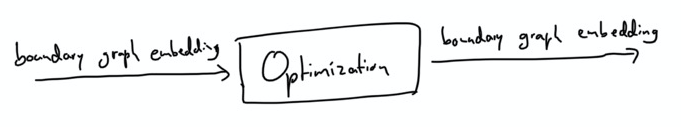
\includegraphics[width=0.9\textwidth]{Resources/Pipeline-Optimization.png}
	\caption{Input and output of the \quoted{Optimization} phase.}
	\label{fig:pipeline-static}
\end{figure}
